% Chapter 3

\chapter{Design and Implementation} % Main chapter title

\label{Chapter3} % For referencing the chapter elsewhere, use \ref{Chapter1} 

%----------------------------------------------------------------------------------------

%----------------------------------------------------------------------------------------

% \section{Image adjustments and Preprocessing methods}
% \subsection{Background segmentation}
% \subsection{Grayscale}
% \subsection{Annotation of Diseased areas}
% \subsection{Semantic Segmentation}
% \section{Learning Structures}
% \subsection{Convolutional Neural Network}
% \subsection{U-net}
% \subsection{ResNet}

% creating artificial dataset\\
% pipes and filters\\
% identifying the disease--|\\
% extracting the disease---|\\
% orientating the disease---algorithm for identifying the parameters for finding the orientation\\

% \begin{figure}[!htb]
%     % \centering
%     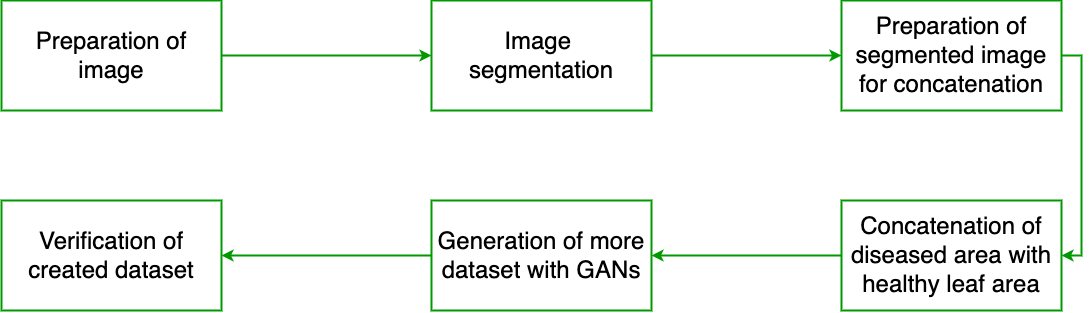
\includegraphics[scale=0.4, keepaspectratio]{Figures/block_diagram v2.png}
%     \caption{Abstract flow of the overall system block diagram of the overall system}
%     \label{fig:my_gan}
% \end{figure}

% \begin{figure}[!htb]
%     \centering
%     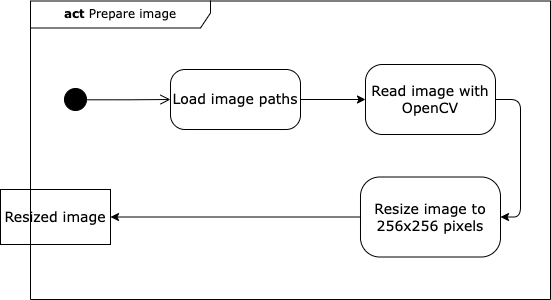
\includegraphics[scale=0.75, keepaspectratio]{Figures/act1.png}
%     \caption{Sample image from the image folder}
%     \label{fig:my_gan}
% \end{figure}


% \begin{figure}[!htb]
%     \centering
%     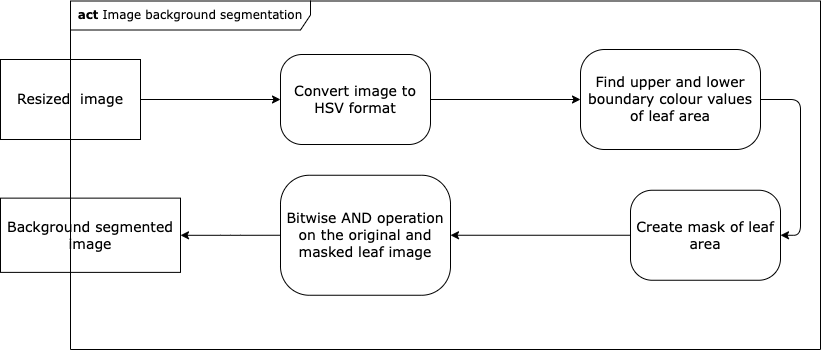
\includegraphics[scale=0.55, keepaspectratio]{Figures/act2.png}
%     \caption{Sample image from the image folder}
%     \label{fig:my_gan}
% \end{figure}


% \begin{figure}[!htb]
%     \centering
%     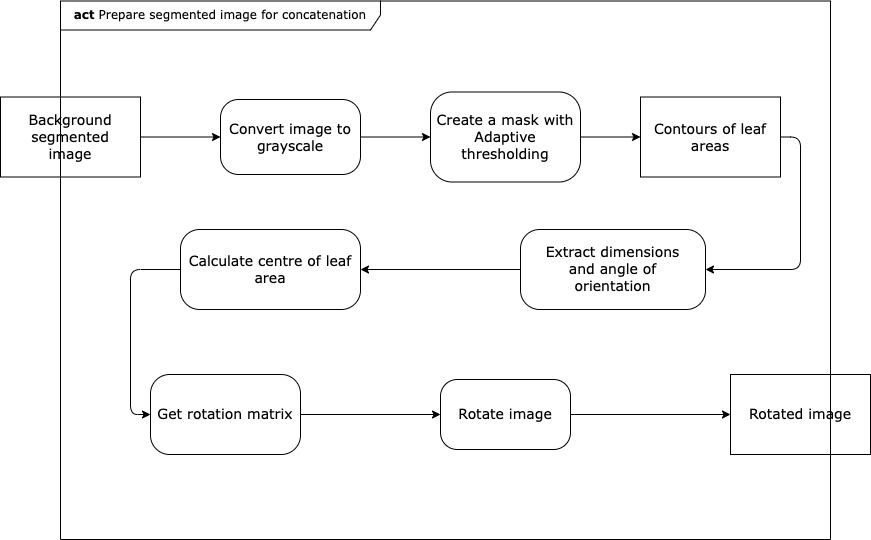
\includegraphics[scale=0.55, keepaspectratio]{Figures/act3.png}
%     \caption{Sample image from the image folder}
%     \label{fig:my_gan}
% \end{figure}

% \begin{figure}[!htb]
%     \centering
%     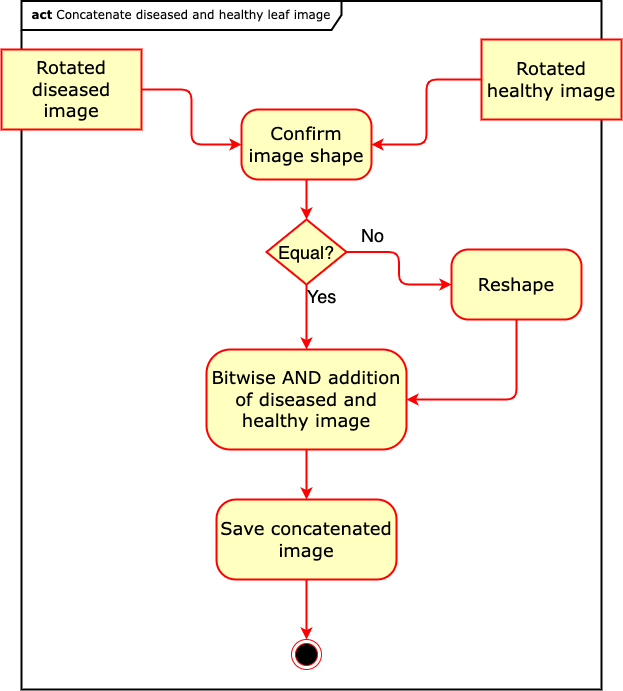
\includegraphics[scale=0.75, keepaspectratio]{Figures/act4.png}
%     \caption{Sample image from the image folder}
%     \label{fig:my_gan}
% \end{figure}

% creating artificial dataset\\
% pipes and filters\\
% identifying the disease--|\\
% extracting the disease---|\\
% orientating the disease---algorithm for identifying the parameters for finding the orientation\\

This chapter discusses the details of the implementation and the reasoning behind some of those choices. This chapter explains the implementation details of foreground and background image segmentation, region of interest (ROI) segmentation, image rotation and colour transformation for artificial disease image dataset. Figure \ref{fig:my_abs_block} shows an abstract block diagram of the flow of approaches for implementing the proposed methodology, with each block in the diagram discussed in the sections below. 
The operations in the first three blocks in figure \ref{fig:my_abs_block} were performed on both the diseased and healthy leaf dataset.
\begin{figure}[!htb]
    % \centering
    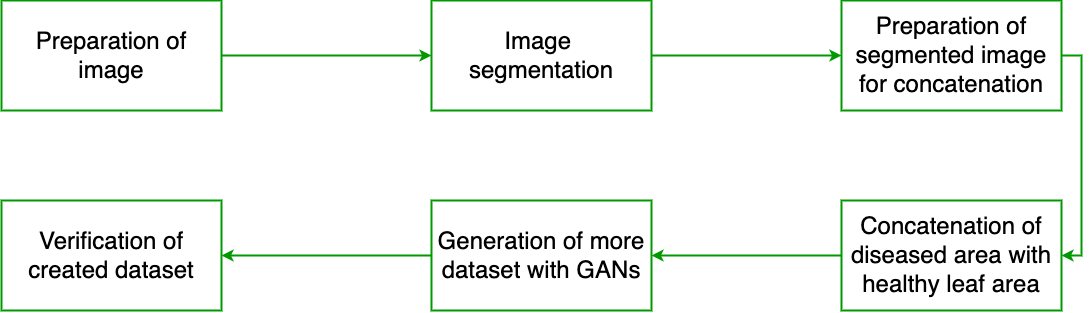
\includegraphics[scale=0.4, keepaspectratio]{Figures/block_diagram v2.png}
    \caption{Abstract flow of the overall system block diagram of the overall system}
    \label{fig:my_abs_block}
\end{figure}

\section{Choice of programming language and library}
OpenCV 2 and Python 3 programming language are used to implement image processing in this research work. The reason for using Python is its comprehensive and efficient use in image processing tasks due to its excellent libraries and tools collections. Likewise, OpenCV was used due to its optimised implementation of several scientifically proven algorithms for image processing and machine learning tasks. Furthermore, through its library, OpenCV provides easy to use methods in Python for image processing tasks like image segmentation, colour transformations and performing thresholding on images. 

\section{Datasets}
The publicly available PlantVillage \cite{hughes2015open} and Plant seedlings \cite{Giselsson2017} datasets were used for the experiment in this thesis. The Plant Seedlings dataset contains images of approximately 960 unique plants belonging to 12 species at several growth stages. The dataset was captured at the Aarhus University Flakkebjerg Research station in collaboration with the University of Southern Denmark and Aarhus University. In contrast, the PlantVillage dataset consists of 54,323 images divided into 38 diseased and healthy plants based on 14 different plant species. All images are taken as a single leaf on a solid background labelled only by a class name.

For creating the artificial dataset, we used 463 images of sugar beet in the plant seedlings dataset as a healthy leaf dataset and 513 images of corn leaves infected with GLS in the PlantVillage dataset as the diseased dataset.
Corn leaves infected with grey leaf spot (GLS caused by \textit{Cercospora zeae-maydis and Cercospora zeina}) were used since it was the only disease in the PlantVillage dataset sharing the same genus ($Cercospora$) of foliar \textit{Cercospora leaf spot (CLS)} caused by \textit{Cercospora beticola}. Figure \ref{fig:my_dis3} and \ref{fig:my_sb_2} show some images of $Corn$ leaves infected with GLS in the PlantVillage dataset and sugar beet leaves in the Plant seedling dataset, respectively. 


\begin{figure}[!htb]
    \centering
    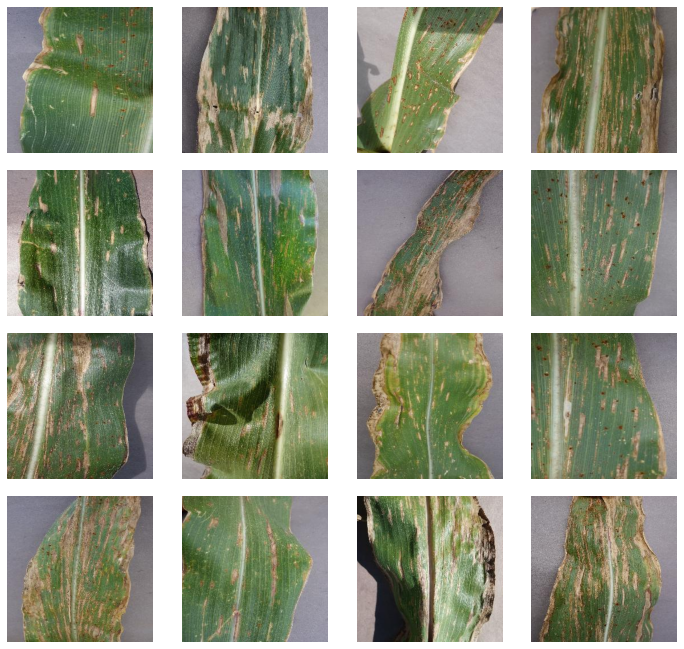
\includegraphics[scale=0.65, keepaspectratio]{Template/Figures/notebook/dis3.png}
    \caption{Activity diagram for image preparation}
    \label{fig:my_dis3}
\end{figure}

\begin{figure}[!htb]
    \centering
    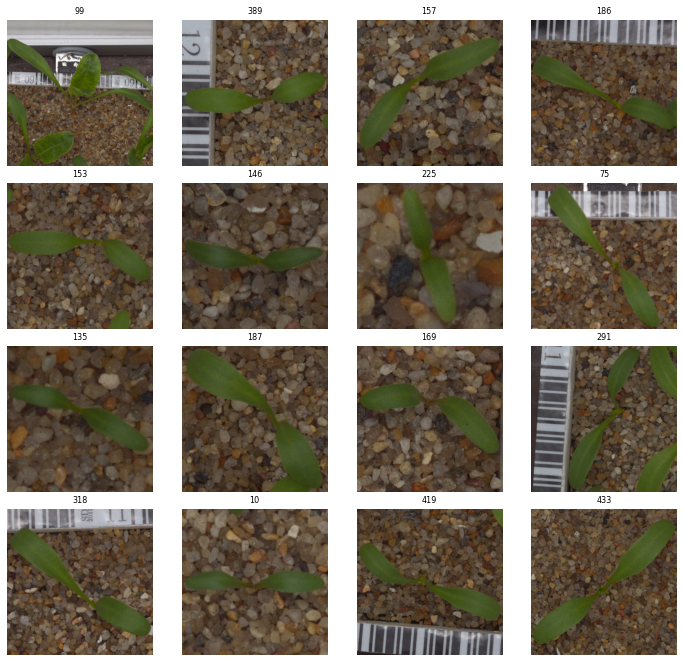
\includegraphics[scale=0.65, keepaspectratio]{Template/Figures/notebook/sb-2.png}
    \caption{Activity diagram for image preparation}
    \label{fig:my_sb_2}
\end{figure}


\section{Image Preparation}
Since the datasets consist of images of different sizes, resizing the images to the same size needs to be done to ensure uniformity in the datasets and allow for a successful addition of the healthy and diseased image dataset since images have to be of the same size. The activity diagram in figure \ref{fig:my_act1} shows the complete control flow of operations in preparing the images for image segmentation.  


\begin{figure}[!htb]
    \centering
    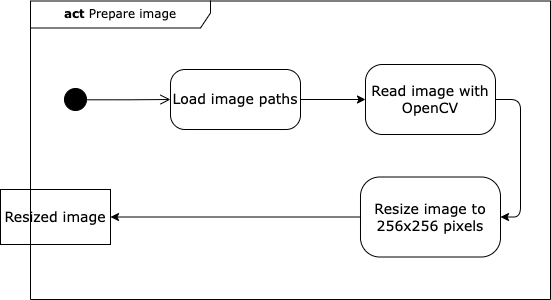
\includegraphics[scale=0.75, keepaspectratio]{Figures/act1.png}
    \caption{Activity diagram for image preparation}
    \label{fig:my_act1}
\end{figure}

The image path of the image to be resized is read using OpenCV. Reading the image with OpenCV allows the capability of resizing the image to 256 x 256 pixels. Furthermore, the resized image is passed on to the image segmentation block in figure \ref{fig:my_abs_block} for further image manipulations.

\section{Image Segmentation}
The leaf areas in images of the diseased and healthy datasets were segmented from their respective backgrounds to reduce the computational complexity of manipulating images with non-uniform backgrounds. Figure \ref{fig:my_act2} shows the flow of actions in segmenting the leaf areas from the background.
\begin{figure}[!htb]
    \centering
    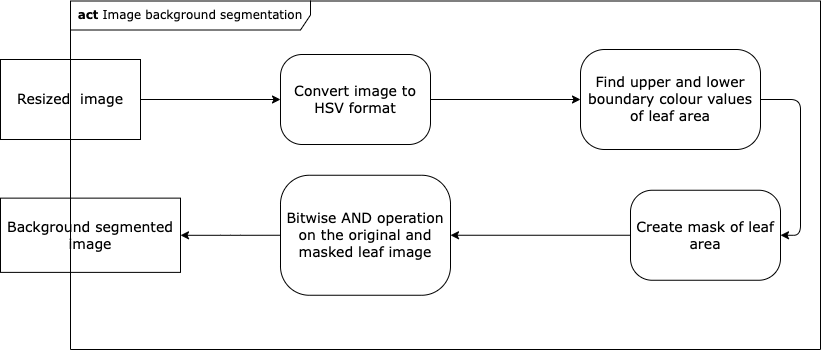
\includegraphics[scale=0.55, keepaspectratio]{Figures/act2.png}
    \caption{Sample image from the image folder}
    \label{fig:my_act2}
\end{figure}

Firstly, the resized image from the previous action is colour transformed from BGR (blue-green-red) into HSV colour space. By default, OpenCV orders the pixels of read images in BGR format. The images were transformed to HSV colour representation because it helps detect green leaf and disease areas in the image. Using the HSV information of the image, the values of the lower and upper boundary representing the green leaf and disease areas in the image were found by splitting and plotting random pixels in the image into its respective hue and saturation values. Figure \ref{fig:my_hsv} show plots of random pixels and the hue and saturation values of random pixels in the PlantVillage dataset. The green clusters represent the leaf area, the brown clusters represent the disease areas and other colour clusters represent other things like specks of dirt and dark background present in the image.

\begin{figure}[!htb]
    \centering
    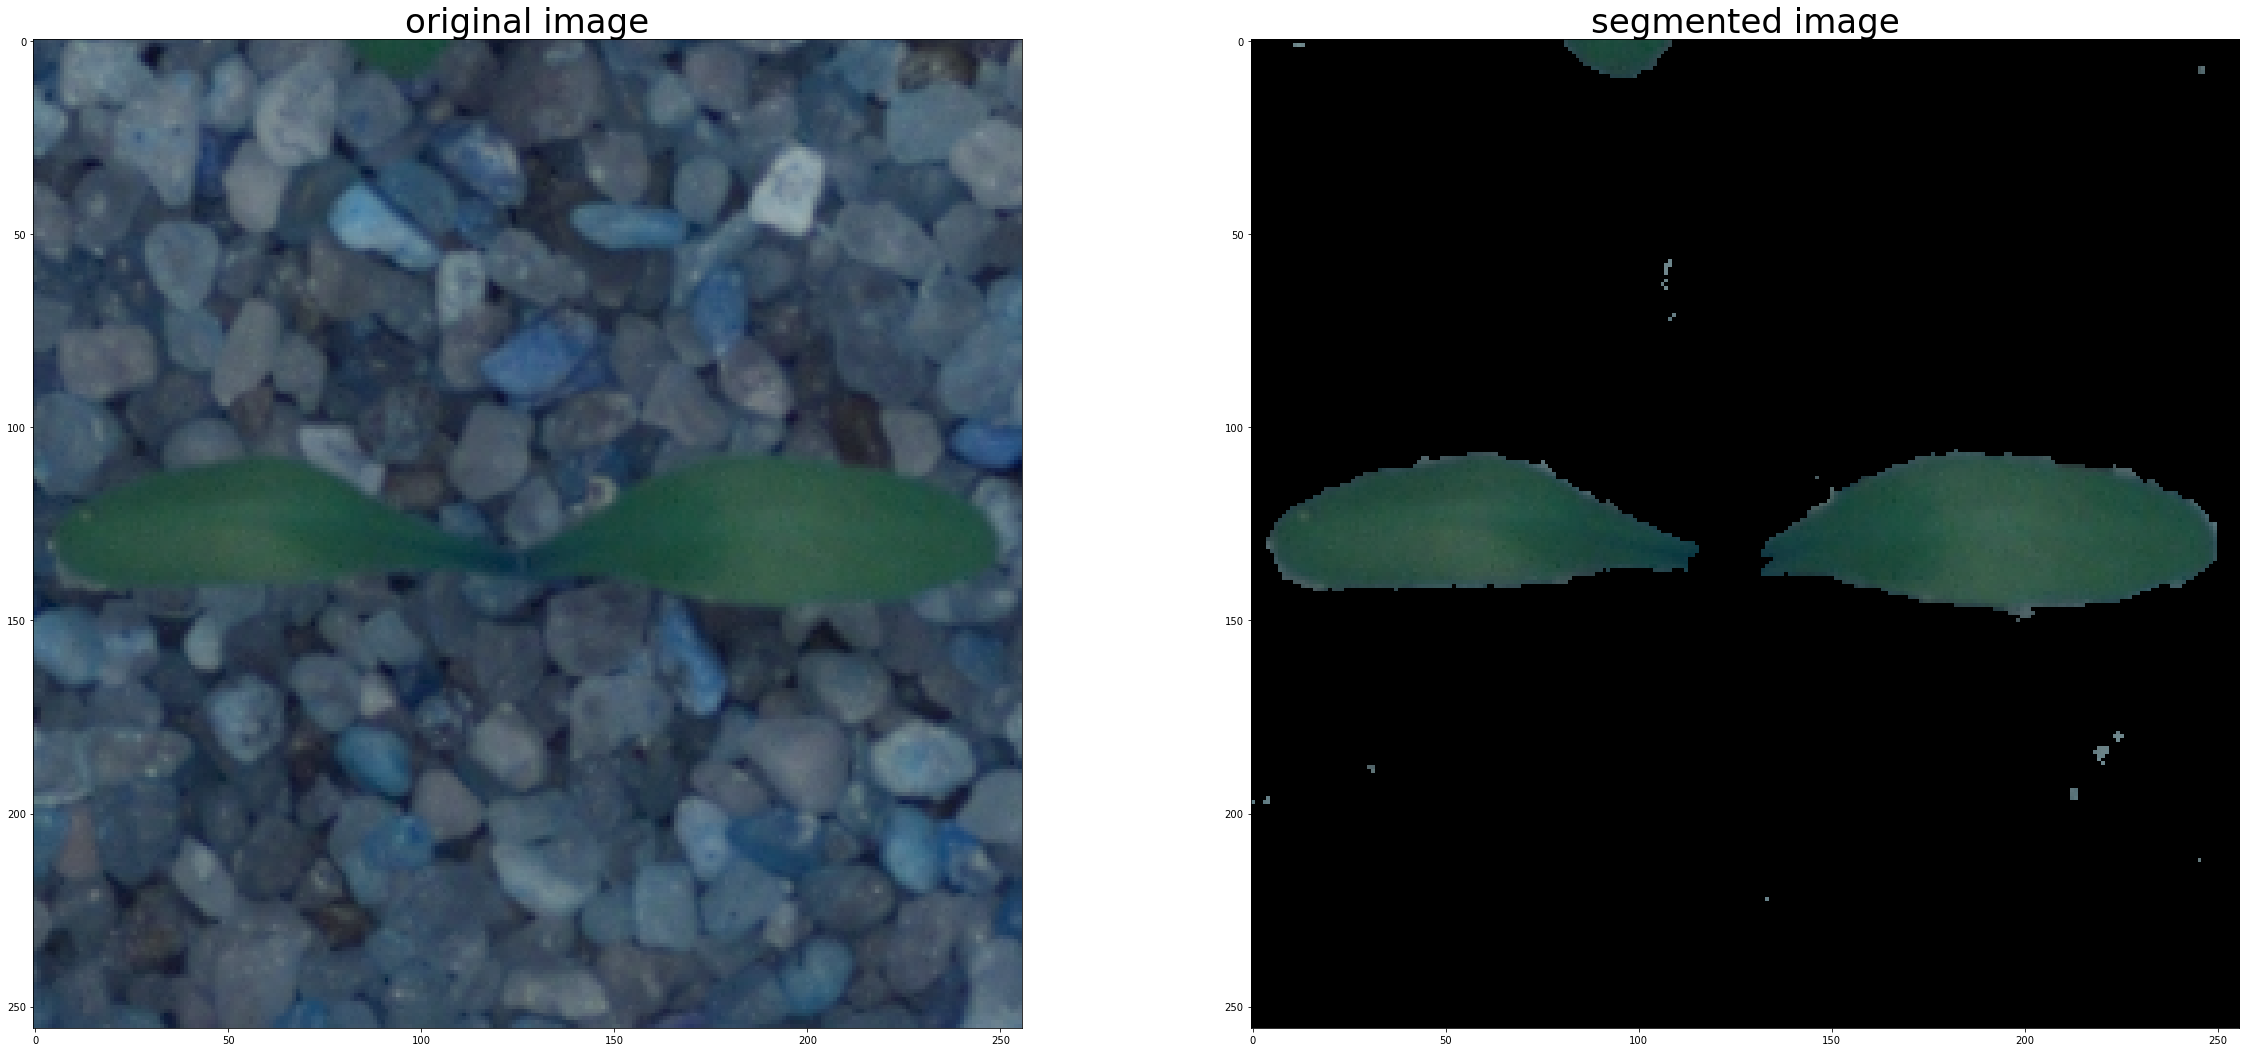
\includegraphics[scale=0.18, keepaspectratio]{Figures/segmen_sugar.png}
    \caption{Sample image from the image folder}
    \label{fig:my_segmen_sugar}
\end{figure}


\begin{figure}[!htb]
    \centering
    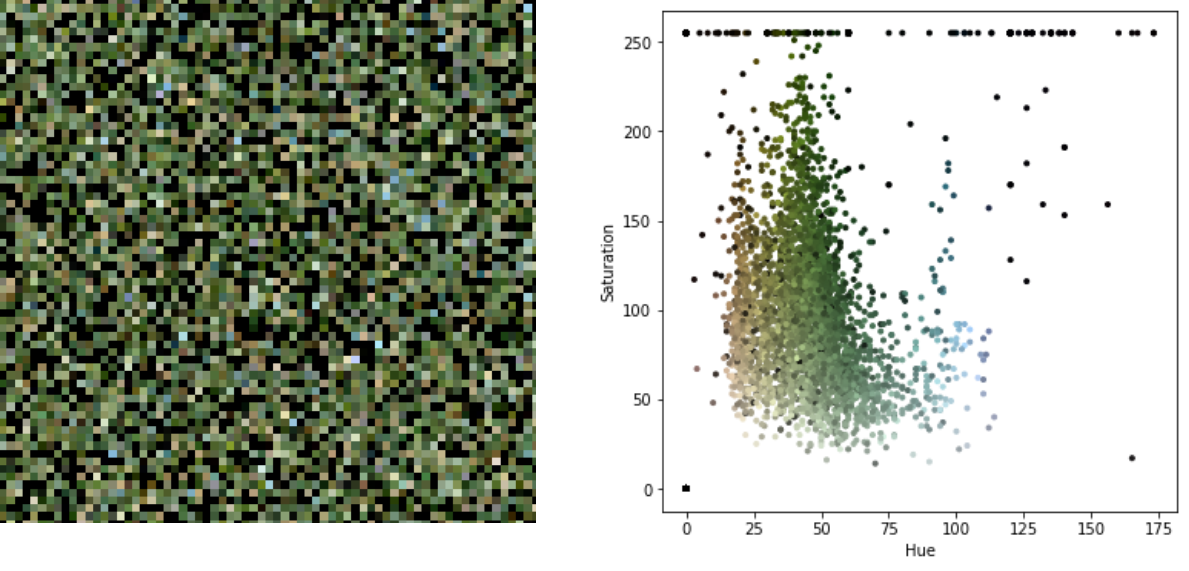
\includegraphics[scale=0.4, keepaspectratio]{Template/Figures/notebook/rand_pixels.png}
    \caption{Sample image from the image folder}
    \label{fig:my_hsv}
\end{figure} 

A mask of the leaf area is created with the found lower and upper boundary HSV value using OpenCV $inRange()$ function. Then, the masked image is used to create a segmented image from the original image using the \textit{bitwise\_AND} operator. Figure \ref{fig:my_segmen_sugar} shows an example of a sugar beet leaf image in the plant seedlings dataset and the resulting background segmented image. Finally, the segmented image is passed on to the next block of actions for further image processing in the section below.

\newpage
\section{Prepare segmented image for Concatenation}
In this section, the actions depicted in figure \ref{fig:myact3} are carried out. The main goal of the actions performed in this section is to rotate the leaf or disease areas in the images vertically. Rotating the leaf/disease area in the vertical direction allows for the consistent positioning of the disease/leaf areas in the datasets since they have different orientations. In addition, having the disease and leaf areas in the same direction ensures that a more significant part of the segmented disease area land on the sugar beet leaf area during image concatenation. 
\begin{figure}[!htb]
    \centering
    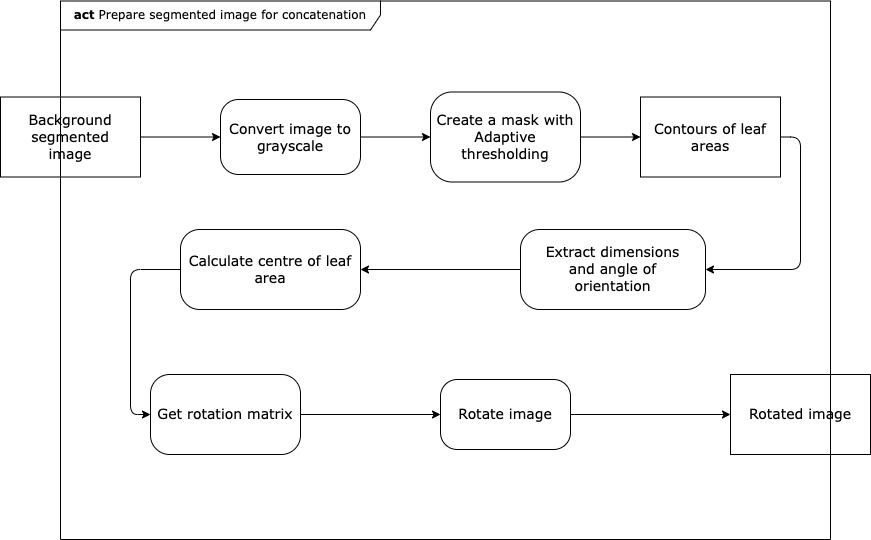
\includegraphics[scale=0.55, keepaspectratio]{Figures/act3.png}
    \caption{Sample image from the image folder}
    \label{fig:myact3}
\end{figure}

As a first step, the segmented image is converted to grayscale. Converting the image to grayscale reduces the dimension of the image to an 8-bit single-channel image, which allows easier manipulations than RGB images which holds the information of all three channels. Equation \ref{color_grey_eqn} is used for the colour to grayscale algorithm implementation in OpenCV.


\begin{equation} \label{color_grey_eqn}
Y = 0.299 R + 0.587 G + 0.114 B
\end{equation}


Furthermore, the  methods \textit{cv2.ADAPTIVE\_THRESH\_MEAN\_C} and\\ \textit{cv2.THRESH\_BINARY\_INV} available in OpenCV was used to create an adaptive threshold binary image of the segmented input image. Binarizing the image enabled us to find the curve joining all the continuous areas along the external boundary of the leaf area since they have the same intensity and colour, i.e. white. Finding the contours of the object of interest in the image gives access to the object’s width, height, length, and orientation angle with respect to the whole image.

The values of the contours of the object of interest were then used to calculate the object’s width, height, length and orientation angle by drawing a minimum area rectangle around the found leaf area. Since detecting the specific location of the leaf area is an interesting task, the implemented solution is further explained in detail in section \ref{leaf_location}.

Non vertically oriented leaf areas were vertically rotated using wrap affine transformation on the transformation matrix $M$ gotten from the OpenCV function\\ \textit{cv2.getRotationMatrix2D()}. Rotation in opencv is counterclockwise ( i.e. positive degrees specify counterclockwise rotation while negative degrees specify clockwise rotation).The transformation matrix $M$ is defined by equation \ref{rota_eqn}


\begin{equation} \label{rota_eqn}
M = 
\begin{bmatrix}
\alpha & \beta & (1-\alpha).c_x -\beta.c_y\\
-\beta & \alpha & \beta.c_x+(1-\alpha).c_y
\end{bmatrix}
\end{equation}

where $ \alpha = scale.\cos{\theta}$, $\beta = scale.\sin{\theta}$, $c_x$  and $c_y$ are the x and y coordinates of the centre of the image and $scale$ is the isotropic scale factor. 

Finally, the vertically rotated image is passed on to the next block for concatenation operation discussed in the next section.

\section{Concatenation of disease area with healthy leaf area}
Before concatenating the segmented disease and healthy leaf image, there needs to be a confirmation that the images are of the same dimensions (i.e. 256 x 256). Inequality in the size of the images will lead to an error. Figure \ref{fig:my_act4} shows the activity diagram of operations in this section.

A region of interest ROI is created on the rotated sugar beet image using the total rows and columns of the disease image. The created ROI of interest has the same size as the disease image since they have the same sizes. Using the disease image, disease areas only corresponding to the leaf regions were extracted using $bitwise\_and$ operation as shown in figure \ref{fig:my_blackout}b. The bitwise addition decides the pixels to be displayed using an AND operation on each pixel of the images (i.e. a bitwise AND operation is true if and only if both pixels are greater than zero). Next, a mask of the disease is created by converting the diseased image to grayscale and then thresholding the grayscale image using $thresh\_binary$. Then an inverse of the mask is created using the $bitwise\_not$ operation. The inverse mask is used to create areas where the disease will fall on in the leaf area. Then, this region of disease on the sugar beet leaf is blacked out using the inverse mask and $bitwise\_operation$ as shown in figure \ref{fig:my_blackout}a.
Finally, the blackout ROI on the leaf and extracted disease region were added together.


% The output of our bitwise AND can be seen in Figure \ref{fig:my_blackout}. It can be seen that the disease pixels that do not fall on the leaf area are turned “off”. Using bitwise arithmetic operations is suitable for the desired result since it avoids the change of image colour, which occurs with an ordinary image addition or the transparent effect that occurs by blending.

\begin{figure}[!htb]
    \centering
    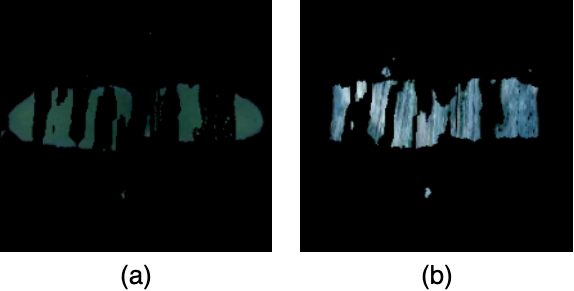
\includegraphics[scale=0.55, keepaspectratio]{Template/Figures/notebook/blackedout.png}
    \caption{Sample image from the image folder}
    \label{fig:my_blackout}
\end{figure} 

\begin{figure}[!htb]
    \centering
    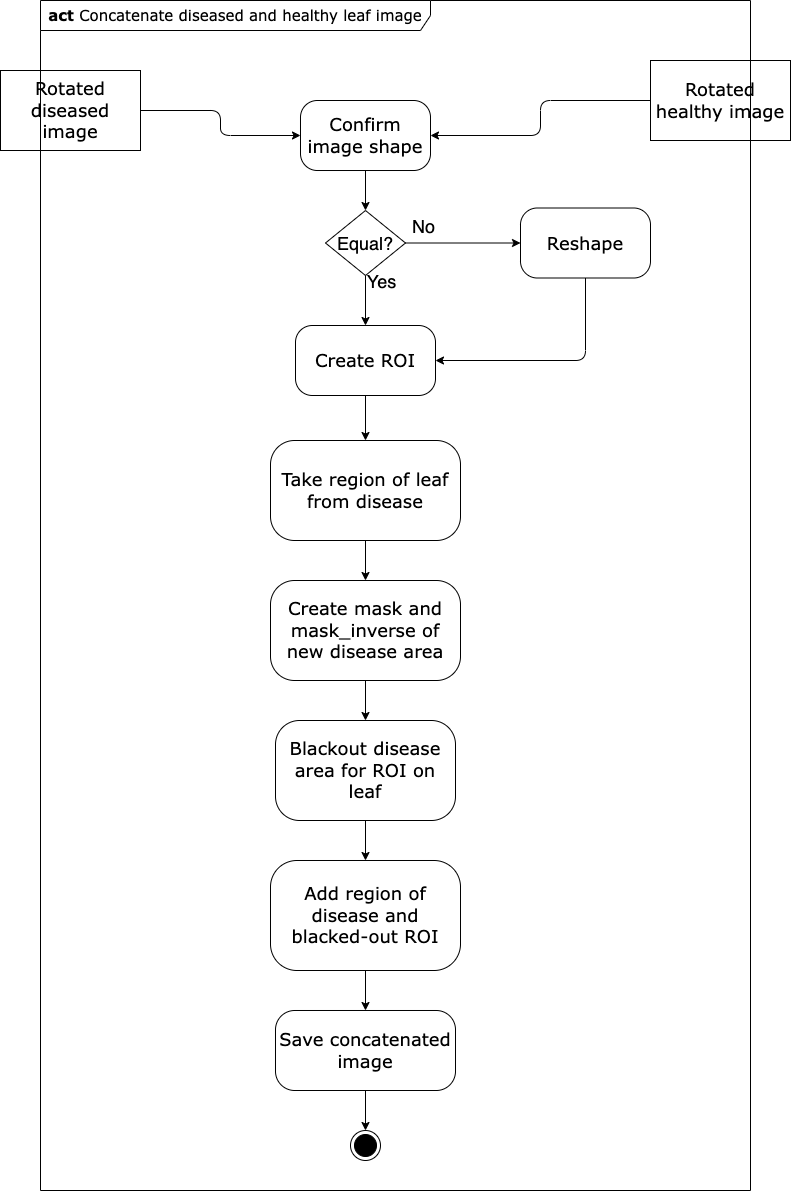
\includegraphics[scale=0.55, keepaspectratio]{Figures/act4.1.png}
    \caption{Sample image from the image folder}
    \label{fig:my_act4}
\end{figure} 
More realistic synthetic diseased leaf datasets can be created using generative adversarial networks. This idea is to train a GANs based model using the generated images from the image manipulation techniques previously discussed. Then, the trained GANs model can be used to create arbitrary values of unique diseased leaf images that could be used in the training phase of a plant disease classifier model. 

Of the GANs based architectures, style GANs have shown promising results in creating higher resolution images of size 256 x 256, ideal for training a CNN-based model. In addition, the Style GANs architecture combines the proGAN and neural style transfer networks for creating new datasets.




% \begin{figure}[!htb]
%     \centering
%     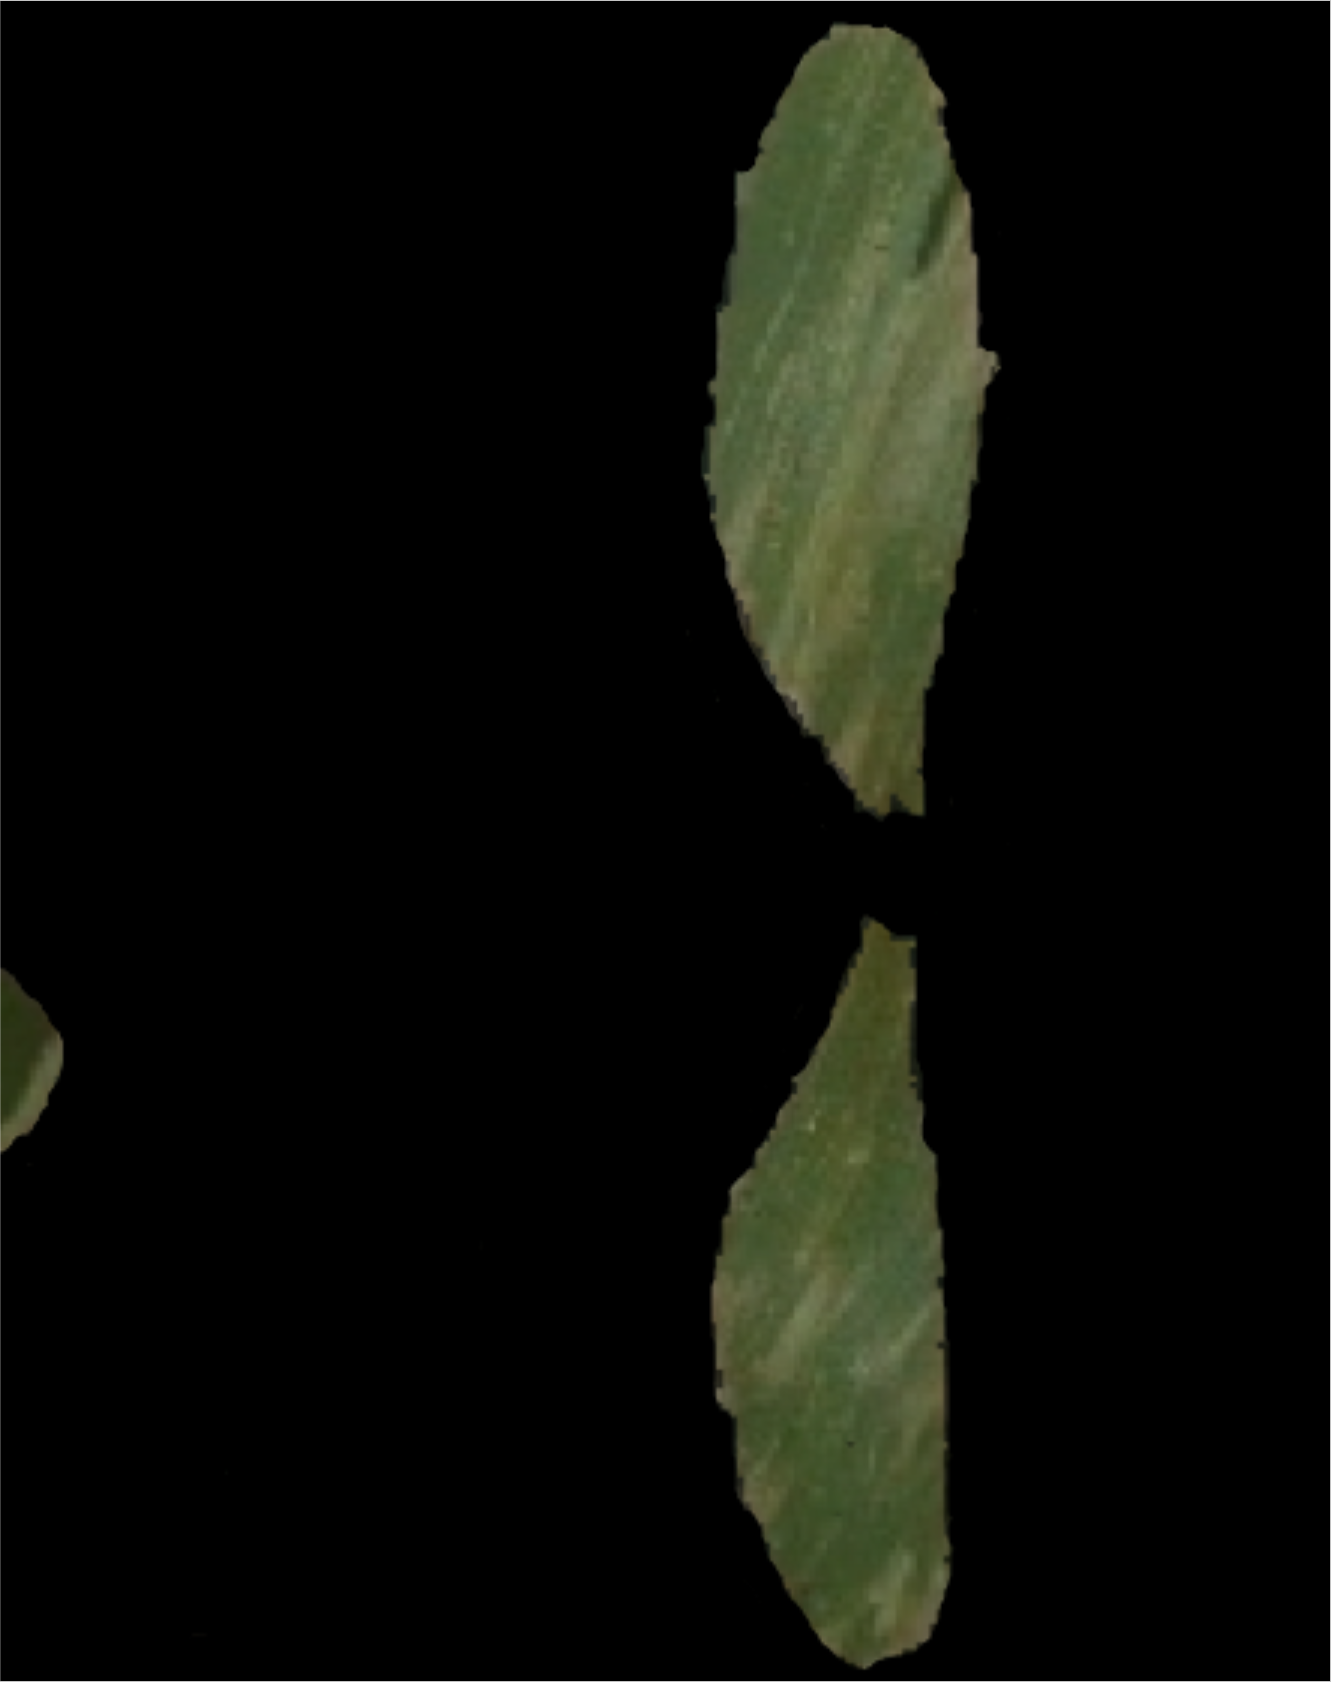
\includegraphics[scale=0.15, keepaspectratio]{Figures/concatenated image.png}
%     \caption{Sample image from the image folder}
%     \label{fig:my_concat}
% \end{figure} 

\section{Detecting Location of Leaf Area in Image}\label{leaf_location}
Contours are curves joining all the continuous areas along the external boundary of objects in an image with the same intensity and colour (i.e. white and black for binary image). For example, the red lines drawn around the detected leaf area in figure \ref{fig:my_cont_rota} shows an example of contours. Contours are helpful for object detection and shape analysis tasks in image processing.
\begin{figure}[!htb]
    \centering
    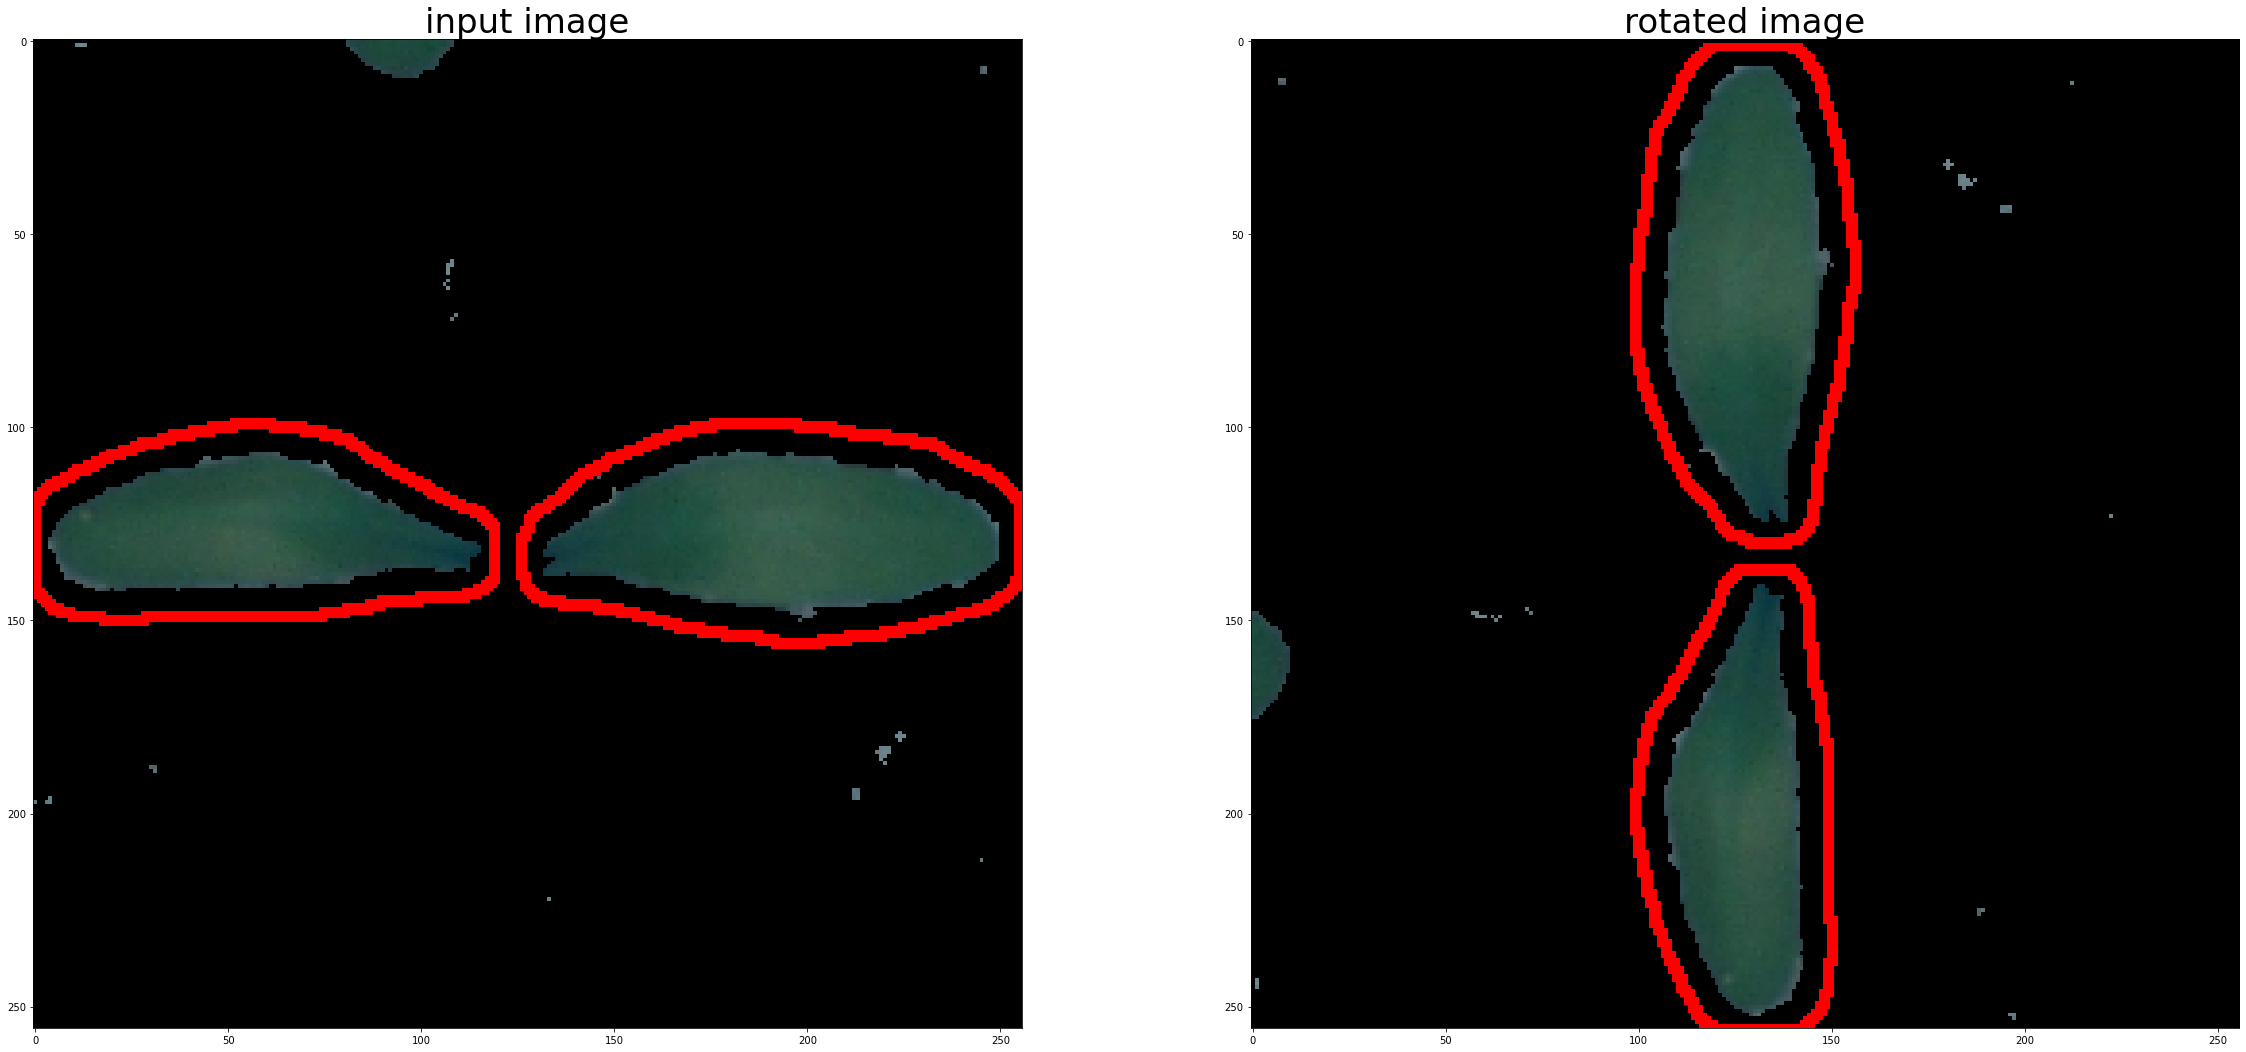
\includegraphics[scale=0.15, keepaspectratio]{Figures/contour.png}
    \caption{Sample image from the image folder}
    \label{fig:my_cont_rota}
\end{figure} 
\begin{figure}[!htb]
    \centering
    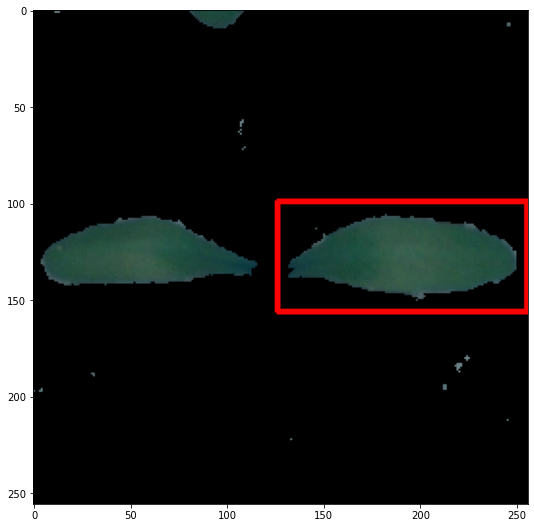
\includegraphics[scale=0.45, keepaspectratio]{Figures/min_rect.png}
    \caption{Sample image from the image folder}
    \label{fig:my_min_rect}
\end{figure} 

The $cv2.findContours()$ function provided by the OpenCV python library provides an implementation for easily detecting objects in an image. The function takes a binary image, contour retrieval mode and approximation method as arguments. Note that Opencv requires that objects of interest in the binary image are white and the background is black. For this experiment, the following were passed in as arguments; the binary image of the leaf, $RETR\_EXTERNAL$ as the retrieval mode (this extracts just the outer contours of the leaf) and $CHAIN\_APPROX\_SIMPLE$ as the approximation method (stores only the coordinates of the object boundary shape). Figure \ref{fig:my_detect_obj} shows the programmatic implementation for finding the contours using Opencv 2 and python 3.
\begin{figure}[!htb]
    \centering
    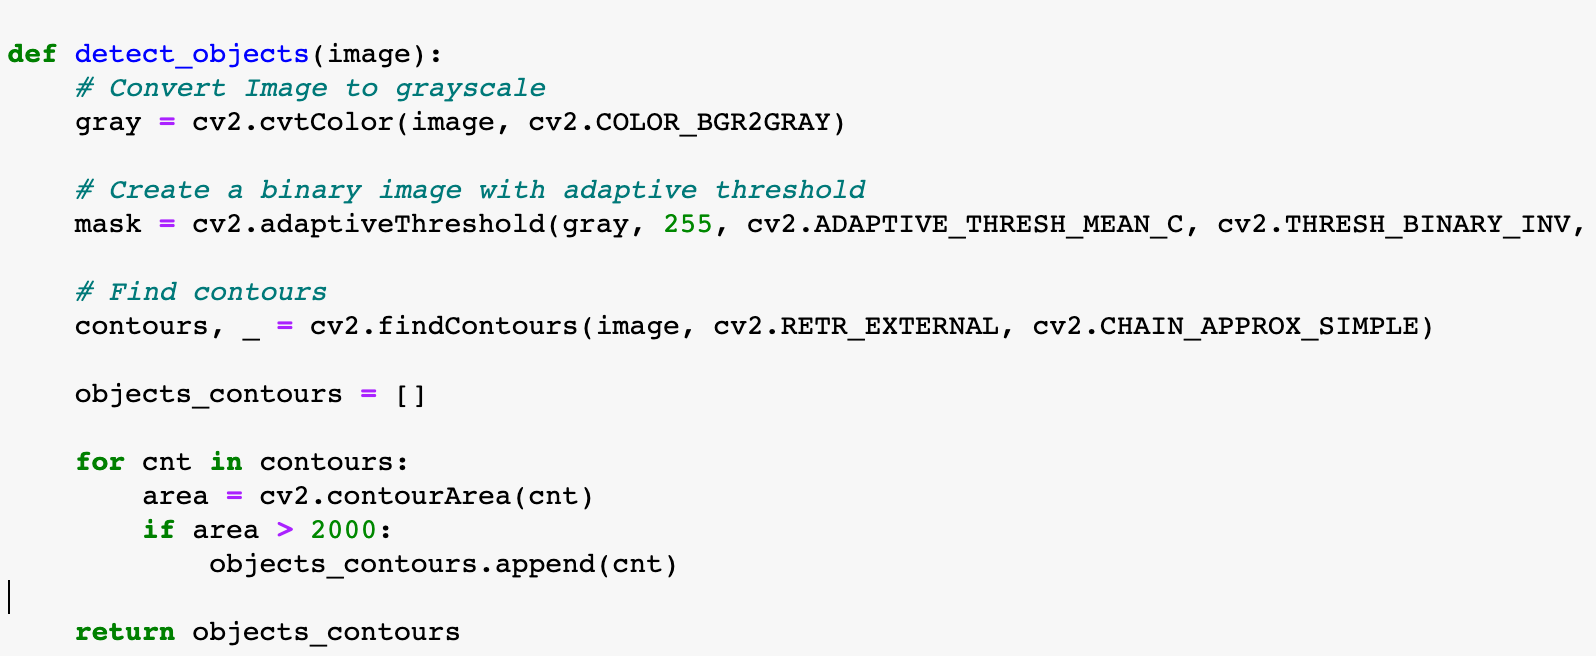
\includegraphics[scale=0.55, keepaspectratio]{Figures/detect_obj.png}
    \caption{Sample image from the image folder}
    \label{fig:my_detect_obj}
\end{figure} 

The contours of binary images are calculated in OpenCV using the algorithm described in \cite{whyna}. The $findContours()$ function in OpenCV returns the modified binary image, hierarchy and contours as a python list (which we are interested in) where each contour is an x and y coordinates of boundary points. 
Every contour whose area is less than 2000 is dropped from the contours list since those values represent non-ROI.
% Since non-ROI have been blacked out, the leaf area will be the only contours in the list.


The values of each contour in the new list can be looped through to create a visual line around the boundaries of the detected leaf object using the $cv2\_polylines()$ function in OpenCV. The lines around the detected leaf region are marked as red in figure \ref{fig:my_cont_rota}. 

Figure \ref{fig:my_find_orien_rotate} shows a code snippet of a helper function that is used to find the angle of orientation of the detected leaf area. The function uses the first contour information passed in as arguments to find its minimum area rotated rectangle. The minimum area rotated rectangle is a bounding rectangle drawn around the detected object to get access to the following details about the object: centre (x, y), (width, height), angle of rotation. Figure \ref{fig:my_min_rect} show the minimum area rectangle of one of the contours of the leaf area. The angle returned by the $findOrientation()$ helper function in figure \ref{fig:my_find_orien_rotate} is then used to rotate the image about its origin using the $rotateImage()$ function shown in figure \ref{fig:my_find_orien_rotate} and the resulting rotated image in figure \ref{fig:my_cont_rota}.


\begin{figure}[!htb]
    \centering
    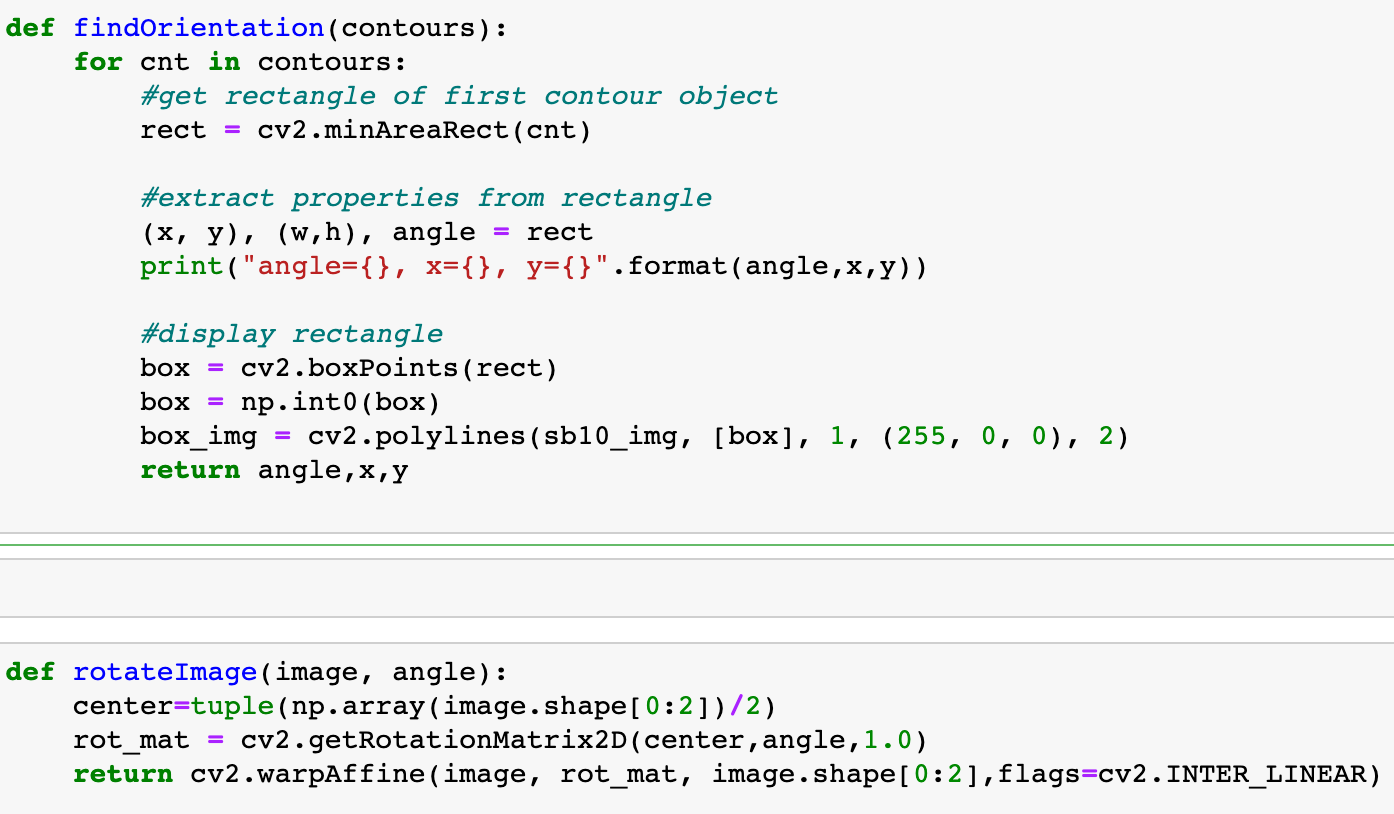
\includegraphics[scale=0.65, keepaspectratio]{Figures/find_orien_rotate.png}
    \caption{Sample image from the image folder}
    \label{fig:my_find_orien_rotate}
\end{figure} 


% \section{Generation of More Dataset with GANs}
% This technique will be theoretically described using scientific references as it was not implemented in this thesis. However, the understandings from this section can be used as a foundation for implementation in future researches.

% Different GAN-based architectures have been developed due to the instability in training models using standard GANs, which often result in ridiculous output by the generator network \cite{radford2015unsupervised}. Therefore, researchers have proposed using other GANs based architectures to create synthetic image datasets to augment currently limited available datasets for training purposes. For example, \cite{gandhi2018plant} used deep convolutional GAN (DCGAN \cite{Radford2015unsupervised}) for creating synthetic images to augment the limited number of local images available for training disease detection models for plants in India. Likewise, \cite{barth2020optimising} in their experiment used Cycle GAN for creating 10 500 synthetic images of bell pepper for their segmentation task, \cite{zhu2018data} created synthetic images from the CVPPP 2017 LSC plant dataset using conditional GAN (CGAN).

% Of all the GAN-based architecture documented in research papers for creating synthetic plant disease images, style GAN has proven to have the best result \cite{arsenovic2019solving}. Style GAN proposed by \cite{karras2019style} combines their previously proposed progressively growing GAN (ProGAN \cite{karras2017progressive}) and neural style transfer (NST \cite{gatys2015neural}) for creating higher resolution (up to 1024 x 1024 pixels) images with features close to the plant leaves. One of the significant advantages of style GAN over standard GAN is its ability to influence details in the style of generated images by changing the values of the style vectors and noise of the network.


% The Style GAN architecture uses its discriminator and generator network to progressively generate synthetic images from a very resolution (4 x 4 pixels) until it reaches the desired target image resolution. The incremental learning allows the network to learn more details about the original images over time. Style GAN replaces the nearest neighbour upsampling layers in the original ProGAN architecture with bilinear sampling. It also uses eight fully connected layers with 512 neurons to process its initial random input.

% Figure \ref{fig:my_style_gan} shows the 256 x 256 pixels synthetic images generated from the PlantVillage dataset by \cite{} using style GAN. Based on the resulting images, it can be concluded that style GAN can be used for generating more synthetic images from the ones created in this thesis.

% \begin{figure}[!htb]
%     \centering
%     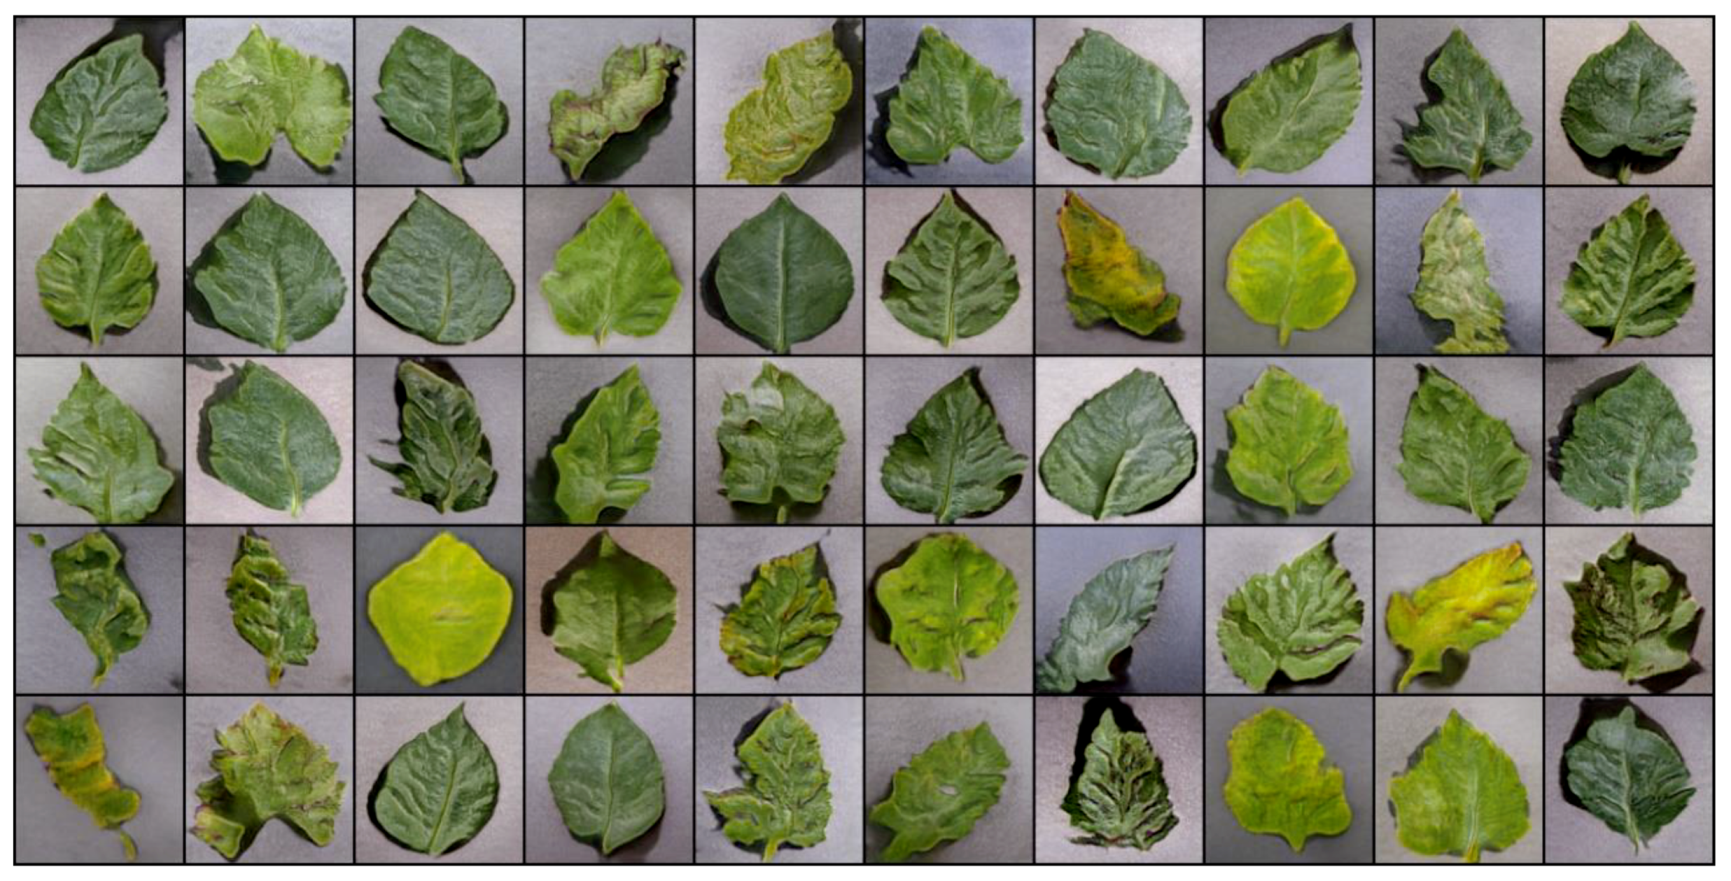
\includegraphics[scale=2, keepaspectratio]{Figures/styleGAN.png}
%     \caption{Sample image from the image folder}
%     \label{fig:my_style_gan}
% \end{figure} 